% !TEX root = ../thesis.tex
\section{Introduction}\label{sec:intro}

There are a multitude of different mathematical knowledge systems and tools. 
A mathematical knowledge system, or MKS, can be defined as a software solution which is aware of (a subset of) mathematical knowledge and can help mathematicians explore a specific field of mathematics. 

These systems can range from calculators, which are only capable of performing simple computations, via mathematical databases (storing a set of a mathematical objects) to powerful modeling tools and computer algebra systems (CAS), that feature a broad variety of features.
A few examples of common MKS include the databases like \cite{oeis} and \cite{lmfdb}, systems like \cite{gap} and \cite{sagemath}, or the Wolfram Mathematica \cite{mathematica11} Computer Algebra System. 

Most of these systems are very specific -- they focus on one or very few aspects of mathematics. 
For example, OEIS is a database of integer sequences and nothing else, 
LMFDB is a database of objects in number theory. 
GAP excels at discrete algebra, whereas SageMath focuses on Algebra and Geometry in general. 

For a mathematician however (a user; let us call her Jane) the systems themselves are not relevant, instead she only cares about being able to solve problems. 
Typically, it is not possible to solve a mathematical problem using only a single problem. 
Thus Jane needs to work with multiple systems and combine the results to reach a solution. 
Currently there is very little help with this practice, so Jane has to isolate sub-problems the respective systems are amenable to, formulate them into the respective input language, collect results, and reformulate them for the next system — a tedious and error-prone process at best, a significant impediment to scientific progress in its overall effect. 
Solutions for some situations certainly exist, which can help get Jane unstuck, but these are ad-hoc and for specific, often-used system combinations only. 
Each of these requires a lot of maintenance and does not scale to a larger set of specialist systems. 

In this thesis, we develop tools and methods of making mathematical software systems interoperable and contribute to a systematic, knowledge-based paradigm for system interoperability -- the \textbf{Math-in-the-Middle (MitM) paradigm} developed in the OpenDreamKit project -- a large-scale project that aims at providing a virtual research environment toolkit for mathematics based on existing (specialist) mathematical software systems. 

In the rest of the introduction, we will briefly review the concepts of the MitM paradigm leading to our research question before we embark in the technical discussion. 

\subsection{The MMT System, Libraries and MathHub}\label{sec:intro:mmt}

The center of the MitM paradigm is the \textbf{Math-in-the-Middle ontology}, a flexiformal representation of mathematical knowledge, which is represented in the the \omdocmmt language, mechanized by the MMT system, and stored in the MathHub information system. 

\mmt\ \cite{Rabe:MMTLanguageSystem09} is a language and framework that was developed to manage (mainly) mathematical knowledge. 
It can handle both formal and informal content. 
\mmt\ is under active development and the project home page can be found at \cite{uniformal:on}. 

Knowledge inside of \mmt\ employs the theory graph paradigm supported by the underlying \omdocmmt\ language. 
This means that knowledge is organized in distinct theories which are related by different relations in a graph-like manner. 
One of these relations is a so-called view, which can be used to translate knowledge from one theory to another. 
Definiens within each theory are identified by a URI (the so-called \mmt\ URI) whereas the definitions are represented by what amounts to OpenMath \cite{BusCapCar:oms04} objects. 
Apart from making purely formal declarations, it is also possible to annotate the declarations with human-readable, narrative elements. 

Commonly all knowledge in \mmt\ is manifested on disk and loaded by the system in its entirety on startup. 
This means that there is a set of files, specifically XML files, on disk containing the appropriate theories and declarations. 
We refer to theories stored in this form as \textit{concrete theories}. 

Knowledge in \mmt can be accessed by either giving it's name -- i.e. it's \mmt\ URI, 
or by giving a set of conditions that has to fulfilled by the knowledge in question. 
The achieve the latter, \mmt has a Query Language called QMT, which allows even complex conditions to be specified. 

This modeling of mathematical knowledge has proven very effective. 
On top of pure mathematical knowledge modeling, it is also possible to annotate declarations. 
This means one can give them human-readable descriptions.
The other direction, giving informal knowledge (for example a paper) a partially formal meaning is also possible.

This has allowed us to develop and populate a system called MathHub \cite{MathHub:on}. 
The system altogether forms a big theory graph totaling at about 10000 theories. 
MathHub is far more than just a theory graph however, it allows creating and editing of existing libraries and offers possibilities for integrating semantic services.
The deatils of this are not relevant to the topic at hand -- we refer the interested reader to \cite{Iancu:phd} instead.

Notable projects available on MathHub include SMGloM \cite{SMGloM:on} -- a semantic glossary of mathematical knowledge -- LATIN \cite{LATIN:online} -- a logical atlas of several different formalizations  -- as well as parts of the PVS \cite{PVSlibraries:on}, MiZar \cite{mizar:online} and HOL Light \cite{KalRab:hollight:14} libraries.

\subsection{Existing Ad-Hoc Solutions for System Interaction}\label{sec:intro:interact}

With the exception of Mathematica none of the previously mentioned systems attempt to be universal -- they do not try to model mathematics as a whole. 
Their focus on specific topics enables them to make concrete optimizations and provide detailed implementations of specific solutions. 

As a result, these systems work very differently -- for example databases only contain a fixed set of objects whereas computer algebra systems commonly allow for complicated manipulation of complex objects. 
This initially limits the inter actability of these systems, and makes it difficult for them to work together. 
Nonetheless, ad-hoc solutions exist and we proceed by giving the reader a brief overview. 

The situation is best illustrated by an example. 
Consider again our user Jane. 
She wishes to check the hypothesis that all abelian transitive groups are cyclic.
How can she go about verifying this hypothesis experimentally with the help of different MKS?

Jane realizes that the \lmfdb\ database contains a set of known abelian transitive groups. 
Furthermore, she realizes that the GAP system can check if a given group is cyclic. 
To check her hypothesis, she could first retrieve all relevant groups from \lmfdb, and then use GAP to check if each of these is cyclic. 
While a positive result would not formally prove her claim, it would certainly give her experimental evidence and show that she should try to prove this formally. 

\input{figs/classicalconnect.tex}
How is such cross-system communication achieved in practice?
\lmfdb\ has implemented an export functionality of the database. 
Each time new data is available in \lmfdb\ it is exported and included in the SageMath software distribution. 
Within SageMath, Jane is provided with a low-level API that can then be used to access this dump. 

To communicate with GAP, a similar approach is chosen. 
A version of GAP is included within Sage, providing a GAP prompt. 
Again, Jane is provided with an interface to make use of GAP commands from within Sage. 

Jane has to first use the \lmfdb\ interface to find all abelian transitive groups. 
This means figuring out how \lmfdb\ works and then manually transferring the objects from \lmfdb\ to Sage. 
Next, she has to make sure that these objects are in a representation that GAP can understand. 
After some translation work, she can then open the GAP prompt in Sage and check for each group if GAP thinks it is cyclic. 

This is obviously a very tedious approach that can easily lead to mistakes. 
It also suffers from many other problems. 
\begin{description}
  \item[Semantic-less interfaces]
  When stating that \lmfdb\ it is exported and included in the SageMath software distribution describes the level of integration well. 
  The semantics of \lmfdb\ are not maintained during this process. 
  
  For example, boolean values are commonly represented as integers $1$ or $0$ in \lmfdb. 
  When accessing the same value from SageMath, no conversion into a SageMath boolean (which is in fact just a python object) is performed -- Jane still only sees a $1$ or a $0$. 
  The difference between $1$ and \inlinecode{true} may seem trivial, but this becomes an issue when talking about data types like matrices or vectors. 
  Continuing, Jane needs to know that the \inlinecode{ab} of a group object in \lmfdb\ is $1$ if it is abelian and $0$ if it is not. 
  
  This is not very mathematical, and it requires being familiar with the technical details of how groups are represented inside of \lmfdb. 

  \item[Updating Problem]
  This obviously requires packaging both \lmfdb\ and GAP for usage within Sage. 
  Each time a change is made in either of these systems, they need to be re-packaged and Sage needs to be updated. 
  This gives rise to a version management problem -- the usage of the newest versions of \lmfdb\ or GAP is not automatic --
  and a data duplication issue. 

  \item[Scaling Up]
  How is more complex communication managed?
  
  Imagine a user in GAP suddenly wanting to make use of \lmfdb. 
  This would mean having to add \lmfdb\ to GAP as well. 
  This not only means more data duplication, it also means having to build another bridge between two systems. 
  In general, to enable communication between $n$ systems each pair of systems need to be connected. 
  This means $O(n^2)$ connections need to be built, leading to a situation as in Figure~\ref{fig:classicalconnect}. 
\end{description}

Mathematica, unlike the other systems mentioned here, attempts to be a universal system. 
One one hand this does have the advantage that it can handle a large subset of Mathematics at once. 
On the other hand, by nature of being a commercial product and not an OpenSource effort, it is not entirely clear how interactions between different components are achieved. 
Mathematica is usually not able to connect to other software systems and mathematicians using Mathematica are required to use only tools available natively in the system. 

\subsection{The Math-In-The-Middle Approach}\label{sec:intro:mitm}

Recall that the OpenDreamKit \cite{OpenDreamKit:on} project is an EU-funded project that aims to create Virtual Research Environments enabling mathematicians to make efficient use of existing Open-Source mathematical knowledge systems. 
These systems include the aforementioned Sage, GAP and \lmfdb\ systems, along with others. 

We give a short overview of the OpenDreamKit project and involved systems here. 
For a a comprehensive list of all projects included in the OpenDreamKit project and in particular the Math-In-The-Middle approach we refer the interested reader to the OpenDreamKit project proposal \cite{ODKproposal:on} as well as reports on the Math-In-The-Middle approach \cite{DehKohKon:iop16}.

\input{figs/mitmconnect.tex}
For this thesis, we build on and make use of the Math-In-The-Middle approach, which can be seen in Figure~\ref{fig:mitmconnect}. 
It models the true, underlying mathematical semantics in \mmt\ (blue $S$) and allows translation between this centrally formalized knowledge and the systems on the boundary (capital letters $A$ - $H$).
This mathematical knowledge is modeled using the well-established theory graph paradigm and is stored inside our MathHub / \mmt\ architecture. 

The knowledge in the systems themselves is also modeled via theories in a theory graph (small letters $a$ - $h$).
This allows us to implement translation with the help of bi-views -- views in both directions -- between the central knowledge -- the Math-In-The-Middle -- and each of the systems. 

Using this mechanism leaves the semantics of translated objects intact -- thus solving the first of the disadvantages listed above. 
Furthermore, when adding a new system it is only required to add $2$ new translations, one from the central math ontology to the system and one in the other direction. 
This drastically reduces the scaling problem -- suddenly only $O(n)$ translations are needed when connecting $n$ different systems. 

\subsection{Research Question}\label{sec:intro:rq}

This leads to our research question. 
How can different mathematical knowledge systems be connected in a generic, efficient and scalable manner to enable transparent, semantics-aware, distributed computation?

As we have seen, to solve this question and be semantics-aware it is required to model mathematics independent of the different systems. 
We need to separate the representations of objects inside each of the systems from their mathematical meaning, the semantics. 
This is achieved by using the semantics-aware, scaleable Math-In-The-Middle approach. 

However, the Math-In-The-Middle approach only provides part of the answer to this question. 
A complete solution needs to address three more aspects which are:
\begin{enumerate}[label={(\roman*)}]
  \item \label{intro:rq:vt} a generic mechanism to manage knowledge stored in the systems and keep it in sync with the Math-In-The-Middle ontologies, 
  \item \label{intro:rq:ql} a system-independent query language, capable of allowing users like Jane to transparently formulate computational problems to be solved, and
  \item \label{intro:rq:com} an efficient lower-level communication layer capable of transporting computational tasks and results between systems, allowing the computational tasks defined by the query language to be resolved in a distributed manner. 
\end{enumerate}

In the following, we give a short overview of how our contribution addresses each of them.

\subsection{Contribution: A Knowledge-based Framework for Distributed Computation at the Math-in-the-Middle Level}\label{sec:intro:com}

Recall that QMT is the Query Language of \mmt. 
As such, it was designed to formulate queries about any kind of knowledge inside of theory graphs and especially inside of \omdocmmt. 
It is thus well-suited for aspect~\ref{intro:rq:ql} above -- it can be used to formulate queries in a system-independent fashion. 
During this thesis, we have extended it to better represent computational aspects and improved support for generic knowlege management. 

SCSCP \cite{SCSCP} stands for Symbolic Computation Software Composability Protocol. 
It is an Open Standard which has been adopted by the OpenMath Society and is already in use by some of the systems in the OpenDreamKit project. 
To enable communication between different mathematical systems it uses a Remote Procedure Call Model. 
All objects and procedure calls are represented using OpenMath objects, making it ideal for out situation -- all content is already modeled in \omdocmmt\ using OpenMath. 
Thus we can make use of it to implement aspect~\ref{intro:rq:com}. 

\subsubsection*{External Knowledge and the Concept of Virtual Theories}\label{sec:intro:external}

This leaves just aspect~\ref{intro:rq:vt} unsolved. 
Knowledge inside of \mmt\ comes from different sources. 
Either it is specifically created by authors or, like here, originally resides in some external system like another MKS. 

Commonly, we use an Import/Export metaphor to make such knowledge available to \mmt. 
This means we create an exporter from the external system that turns the knowledge representation of the external system directly into \omdocmmt. 
This knowledge is then stored by the \mmt\ system in a set of XML files representing \omdocmmt. 
These XML files are then used by \mmt\ just like any other concrete theory is used. 

Such a process has proven to be very useful -- it makes all information available to \mmt\ directly. 
In other words, the knowledge is consolidated on the users disk -- and thus it can be accessed even if the original system no longer works. 

This means that any change in the external system requires us to re-import the knowledge -- the same updating problem encountered in Jane's original approach above. 
This is not a scalable solution and thus does not suffice to address this aspect of our research question. 

Instead, we have introduced a second type of theory to \mmt, the so-called virtual theory. 
In a nutshell, virtual theories are just like concrete theories, but without the assumption of loading all declarations from a file on disk at system startup. 
Instead of loading all knowledge from an XML file, virtual theories load declarations in a lazy fashion when they are required. 
Here we do not even restrict ourselves to lazily reading an XML file, on the contrary, in most use cases we actually create the \omdocmmt\ representation on demand. 

Notice that a replacement of the Import/Export metaphor by virtual theories only makes sense in certain situations. 
In the case of \lmfdb, we can easily translate a single declaration, whereas in the case of a theorem prover library like PVS this is not the case. 
Instead of having to start an entire theorem prover system to only load a single declaration, it makes far more sense to import the library as a whole. 

In the architecture needed to solve the research question, it does make sense to use virtual theories. 
virtual theories have the key advantage that we can directly access the knowledge of other systems. 
There is little to no need to manually keep the Math-In-The-Middle ontology in sync -- by use of a virtual theory this happens automatically. 

Our core example for virtual theories is the the \lmfdb\ database introduced above. 
An \lmfdb\ virtual theory can retrieve the content of a single declaration in \lmfdb\ form and proceed to translate it to \omdocmmt. 
Only items explicitly needed by the user or some other process inside of the \mmt\ API need to be retrieved and translated. 

The choice of virtual theories as a solution to aspect~\ref{intro:rq:vt} also has implications for the query layer. 
As it turns out the existing QMT implementation relies on implementation details of concrete theories. 
In particular, it makes the assumption that all queryable knowledge is available inside of \mmt\ memory.
As this does not hold for virtual theories, during the course of this thesis we have had to adapt the implementation accordingly. 

\subsubsection*{Solving Jane's Example}\label{sec:intro:vtuse}

% !TEX root = ../thesis.tex
\begin{figure}[h]
  \begin{center}
    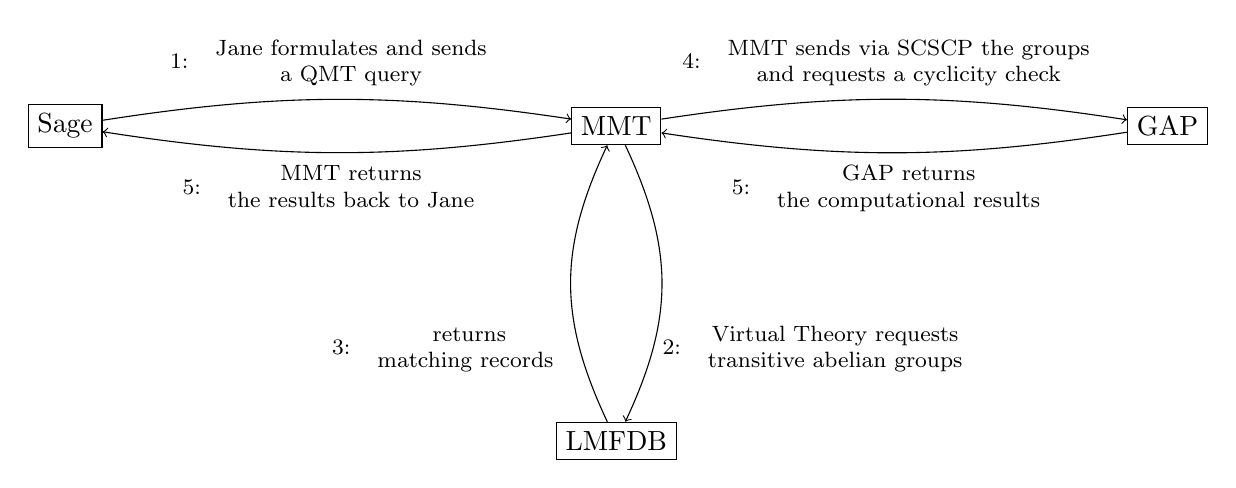
\begin{tikzpicture}[xscale=7,yscale=4]\normalsize
      \node[draw] (s) at (0,0) {Sage};
      \node[draw] (m) at (1,0) {MMT};
      \node[draw] (g) at (2,0) {GAP};
      \node[draw] (l) at (1,-1) {LMFDB};
      \draw[->] (s) to[bend left=15] node[above] {
        \footnotesize 1: 
        \begin{tabular}{c}
          Jane formulates and sends\\
          a QMT query
        \end{tabular}
      } (m);
      \draw[->] (m) to[bend left=15] node[right,near end] {
        \footnotesize 2: 
        \begin{tabular}{c}
          Virtual Theory requests \\
          transitive abelian groups
        \end{tabular}
      } (l);
      \draw[<-] (m) to[bend right=15] node[left,near end] {
        \footnotesize 3: 
        \begin{tabular}{c}
          \lmfdb\ returns\\
          matching records
        \end{tabular}
      } (l);
      \draw[->] (m) to[bend left=15] node[above] {
        \footnotesize 4: 
        \begin{tabular}{c}
          MMT sends via SCSCP the groups\\
          and requests a cyclicity check
        \end{tabular}
      } (g);
      \draw[<-] (m) to[bend right=15] node[below] {
        \footnotesize 5: 
        \begin{tabular}{c}
          GAP returns\\
          the computational results
        \end{tabular}
      } (g);
      \draw[<-] (s) to[bend right=15] node[below] {
        \footnotesize 5: 
        \begin{tabular}{c}
          MMT returns\\
          the results back to Jane
        \end{tabular}
      } (m);
    \end{tikzpicture}
  \end{center}

  \caption[A MiTM use-case]{
    Solving Jane's example of Cross-System Communication using our approach. 
  }
  \label{fig:mitmcaseintro}
\end{figure}
Recall the example involving Jane from above. 
We give a short preview in Figure~\ref{fig:mitmcaseintro} of how our choices to use virtual theories, QMT and SCSCP can be used to solve this use-case. 

Instead of writing all queries in a Sage-specific manner within the Sage System and targeting \lmfdb\ and GAP directly, Jane can make use of the QMT Query Language and send a single query to MMT that expresses the semantics of the information she wishes to retrieve. 

Unlike in existing solutions, she does not have to be aware of the low-level implementation details. 
Instead she can semantically ask for ``abelian groups'' and if a system is ``cyclic'' or not. 
The \mmt\ system will figure out the exact system-specific details using views. 
Furthermore, all the intermediate steps are hidden from Jane's point of view -- she can get her result in a single step instead of the multitude of steps required usually. 

We will come back to this example later -- and discuss it in more detail. 

\subsection{Structure}\label{sec:intro:toc}

We will proceed as follows:
% 2 - MMT
In Section~\ref{sec:mmt} we describe the structure of the \mmt\ system, 
% 3 - Representing Knowledge Using the Math-In-The-Middle Approach
and then continue in Section~\ref{sec:mitm} to describe the Math-In-The-Middle approach and how to utilize it with the Systems found in the OpenDreamKit project. 
% 4 - virtual theories as a Uniform Conceptual Interface for Mathematical Databases
We move on in Section~\ref{sec:vt} to detail our virtual theory implementation and how they function as a uniform conceptual interface to Mathematical Databases. 
% 5 - QMT
Next, in Section~\ref{sec:qmt} we examine the existing implementation and improvements we have made to the QMT Query Language 
% 6 - Communication
and then discuss in Section~\ref{sec:comm} how it is used to enable cross-system communication within our architecture. 
% 6 - Conclusion
Finally we conclude in Section~\ref{sec:conclusion} by revisiting Jane's example and discussing how the progress made during this thesis can be used in cross-system communication. 
We also give a brief outlook. 